% Created by tikzDevice version 0.12.3 on 2019-09-28 00:51:42
% !TEX encoding = UTF-8 Unicode
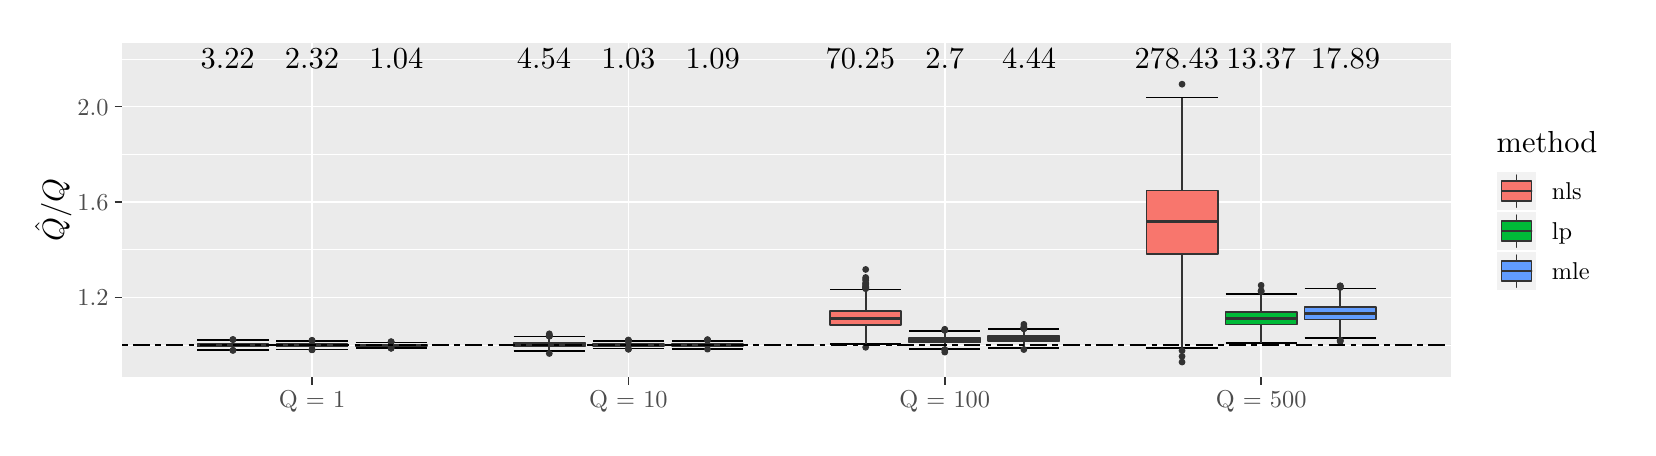
\begin{tikzpicture}[x=1pt,y=1pt]
\definecolor{fillColor}{RGB}{255,255,255}
\path[use as bounding box,fill=fillColor,fill opacity=0.00] (0,0) rectangle (578.16,144.54);
\begin{scope}
\path[clip] (  0.00,  0.00) rectangle (578.16,144.54);
\definecolor{drawColor}{RGB}{255,255,255}
\definecolor{fillColor}{RGB}{255,255,255}

\path[draw=drawColor,line width= 0.6pt,line join=round,line cap=round,fill=fillColor] (  0.00,  0.00) rectangle (578.16,144.54);
\end{scope}
\begin{scope}
\path[clip] ( 34.16, 18.22) rectangle (514.31,139.04);
\definecolor{fillColor}{gray}{0.92}

\path[fill=fillColor] ( 34.16, 18.22) rectangle (514.31,139.04);
\definecolor{drawColor}{RGB}{255,255,255}

\path[draw=drawColor,line width= 0.3pt,line join=round] ( 34.16, 29.82) --
	(514.31, 29.82);

\path[draw=drawColor,line width= 0.3pt,line join=round] ( 34.16, 64.29) --
	(514.31, 64.29);

\path[draw=drawColor,line width= 0.3pt,line join=round] ( 34.16, 98.76) --
	(514.31, 98.76);

\path[draw=drawColor,line width= 0.3pt,line join=round] ( 34.16,133.23) --
	(514.31,133.23);

\path[draw=drawColor,line width= 0.6pt,line join=round] ( 34.16, 47.06) --
	(514.31, 47.06);

\path[draw=drawColor,line width= 0.6pt,line join=round] ( 34.16, 81.53) --
	(514.31, 81.53);

\path[draw=drawColor,line width= 0.6pt,line join=round] ( 34.16,116.00) --
	(514.31,116.00);

\path[draw=drawColor,line width= 0.6pt,line join=round] (102.75, 18.22) --
	(102.75,139.04);

\path[draw=drawColor,line width= 0.6pt,line join=round] (217.07, 18.22) --
	(217.07,139.04);

\path[draw=drawColor,line width= 0.6pt,line join=round] (331.39, 18.22) --
	(331.39,139.04);

\path[draw=drawColor,line width= 0.6pt,line join=round] (445.71, 18.22) --
	(445.71,139.04);
\definecolor{drawColor}{RGB}{0,0,0}

\path[draw=drawColor,line width= 0.6pt,line join=round] ( 61.31, 31.65) --
	( 87.03, 31.65);

\path[draw=drawColor,line width= 0.6pt,line join=round] ( 74.17, 31.65) --
	( 74.17, 28.11);

\path[draw=drawColor,line width= 0.6pt,line join=round] ( 61.31, 28.11) --
	( 87.03, 28.11);

\path[draw=drawColor,line width= 0.6pt,line join=round] ( 89.89, 31.37) --
	(115.61, 31.37);

\path[draw=drawColor,line width= 0.6pt,line join=round] (102.75, 31.37) --
	(102.75, 28.27);

\path[draw=drawColor,line width= 0.6pt,line join=round] ( 89.89, 28.27) --
	(115.61, 28.27);

\path[draw=drawColor,line width= 0.6pt,line join=round] (118.47, 30.82) --
	(144.19, 30.82);

\path[draw=drawColor,line width= 0.6pt,line join=round] (131.33, 30.82) --
	(131.33, 28.82);

\path[draw=drawColor,line width= 0.6pt,line join=round] (118.47, 28.82) --
	(144.19, 28.82);

\path[draw=drawColor,line width= 0.6pt,line join=round] (175.63, 32.98) --
	(201.35, 32.98);

\path[draw=drawColor,line width= 0.6pt,line join=round] (188.49, 32.98) --
	(188.49, 27.59);

\path[draw=drawColor,line width= 0.6pt,line join=round] (175.63, 27.59) --
	(201.35, 27.59);

\path[draw=drawColor,line width= 0.6pt,line join=round] (204.21, 31.29) --
	(229.93, 31.29);

\path[draw=drawColor,line width= 0.6pt,line join=round] (217.07, 31.29) --
	(217.07, 28.60);

\path[draw=drawColor,line width= 0.6pt,line join=round] (204.21, 28.60) --
	(229.93, 28.60);

\path[draw=drawColor,line width= 0.6pt,line join=round] (232.79, 31.30) --
	(258.51, 31.30);

\path[draw=drawColor,line width= 0.6pt,line join=round] (245.65, 31.30) --
	(245.65, 28.44);

\path[draw=drawColor,line width= 0.6pt,line join=round] (232.79, 28.44) --
	(258.51, 28.44);

\path[draw=drawColor,line width= 0.6pt,line join=round] (289.95, 49.91) --
	(315.67, 49.91);

\path[draw=drawColor,line width= 0.6pt,line join=round] (302.81, 49.91) --
	(302.81, 30.15);

\path[draw=drawColor,line width= 0.6pt,line join=round] (289.95, 30.15) --
	(315.67, 30.15);

\path[draw=drawColor,line width= 0.6pt,line join=round] (318.53, 34.96) --
	(344.25, 34.96);

\path[draw=drawColor,line width= 0.6pt,line join=round] (331.39, 34.96) --
	(331.39, 28.33);

\path[draw=drawColor,line width= 0.6pt,line join=round] (318.53, 28.33) --
	(344.25, 28.33);

\path[draw=drawColor,line width= 0.6pt,line join=round] (347.11, 35.54) --
	(372.83, 35.54);

\path[draw=drawColor,line width= 0.6pt,line join=round] (359.97, 35.54) --
	(359.97, 28.74);

\path[draw=drawColor,line width= 0.6pt,line join=round] (347.11, 28.74) --
	(372.83, 28.74);

\path[draw=drawColor,line width= 0.6pt,line join=round] (404.27,119.25) --
	(430.00,119.25);

\path[draw=drawColor,line width= 0.6pt,line join=round] (417.13,119.25) --
	(417.13, 28.69);

\path[draw=drawColor,line width= 0.6pt,line join=round] (404.27, 28.69) --
	(430.00, 28.69);

\path[draw=drawColor,line width= 0.6pt,line join=round] (432.85, 48.28) --
	(458.58, 48.28);

\path[draw=drawColor,line width= 0.6pt,line join=round] (445.71, 48.28) --
	(445.71, 30.56);

\path[draw=drawColor,line width= 0.6pt,line join=round] (432.85, 30.56) --
	(458.58, 30.56);

\path[draw=drawColor,line width= 0.6pt,line join=round] (461.43, 50.24) --
	(487.16, 50.24);

\path[draw=drawColor,line width= 0.6pt,line join=round] (474.29, 50.24) --
	(474.29, 32.36);

\path[draw=drawColor,line width= 0.6pt,line join=round] (461.43, 32.36) --
	(487.16, 32.36);
\definecolor{drawColor}{gray}{0.20}
\definecolor{fillColor}{gray}{0.20}

\path[draw=drawColor,line width= 0.4pt,line join=round,line cap=round,fill=fillColor] ( 74.17, 31.86) circle (  1.02);

\path[draw=drawColor,line width= 0.4pt,line join=round,line cap=round,fill=fillColor] ( 74.17, 27.95) circle (  1.02);

\path[draw=drawColor,line width= 0.4pt,line join=round,line cap=round,fill=fillColor] ( 74.17, 27.94) circle (  1.02);

\path[draw=drawColor,line width= 0.4pt,line join=round,line cap=round,fill=fillColor] ( 74.17, 31.80) circle (  1.02);

\path[draw=drawColor,line width= 0.6pt,line join=round] ( 74.17, 30.27) -- ( 74.17, 31.65);

\path[draw=drawColor,line width= 0.6pt,line join=round] ( 74.17, 29.35) -- ( 74.17, 28.11);
\definecolor{fillColor}{RGB}{248,118,109}

\path[draw=drawColor,line width= 0.6pt,line join=round,line cap=round,fill=fillColor] ( 61.31, 30.27) --
	( 61.31, 29.35) --
	( 87.03, 29.35) --
	( 87.03, 30.27) --
	( 61.31, 30.27) --
	cycle;

\path[draw=drawColor,line width= 1.1pt,line join=round] ( 61.31, 29.79) -- ( 87.03, 29.79);
\definecolor{fillColor}{gray}{0.20}

\path[draw=drawColor,line width= 0.4pt,line join=round,line cap=round,fill=fillColor] (102.75, 28.21) circle (  1.02);

\path[draw=drawColor,line width= 0.4pt,line join=round,line cap=round,fill=fillColor] (102.75, 31.46) circle (  1.02);

\path[draw=drawColor,line width= 0.4pt,line join=round,line cap=round,fill=fillColor] (102.75, 31.59) circle (  1.02);

\path[draw=drawColor,line width= 0.4pt,line join=round,line cap=round,fill=fillColor] (102.75, 28.12) circle (  1.02);

\path[draw=drawColor,line width= 0.4pt,line join=round,line cap=round,fill=fillColor] (102.75, 28.20) circle (  1.02);

\path[draw=drawColor,line width= 0.6pt,line join=round] (102.75, 30.22) -- (102.75, 31.37);

\path[draw=drawColor,line width= 0.6pt,line join=round] (102.75, 29.44) -- (102.75, 28.27);
\definecolor{fillColor}{RGB}{0,186,56}

\path[draw=drawColor,line width= 0.6pt,line join=round,line cap=round,fill=fillColor] ( 89.89, 30.22) --
	( 89.89, 29.44) --
	(115.61, 29.44) --
	(115.61, 30.22) --
	( 89.89, 30.22) --
	cycle;

\path[draw=drawColor,line width= 1.1pt,line join=round] ( 89.89, 29.82) -- (115.61, 29.82);
\definecolor{fillColor}{gray}{0.20}

\path[draw=drawColor,line width= 0.4pt,line join=round,line cap=round,fill=fillColor] (131.33, 28.75) circle (  1.02);

\path[draw=drawColor,line width= 0.4pt,line join=round,line cap=round,fill=fillColor] (131.33, 31.09) circle (  1.02);

\path[draw=drawColor,line width= 0.4pt,line join=round,line cap=round,fill=fillColor] (131.33, 30.93) circle (  1.02);

\path[draw=drawColor,line width= 0.4pt,line join=round,line cap=round,fill=fillColor] (131.33, 30.95) circle (  1.02);

\path[draw=drawColor,line width= 0.4pt,line join=round,line cap=round,fill=fillColor] (131.33, 28.79) circle (  1.02);

\path[draw=drawColor,line width= 0.4pt,line join=round,line cap=round,fill=fillColor] (131.33, 28.69) circle (  1.02);

\path[draw=drawColor,line width= 0.6pt,line join=round] (131.33, 30.08) -- (131.33, 30.82);

\path[draw=drawColor,line width= 0.6pt,line join=round] (131.33, 29.57) -- (131.33, 28.82);
\definecolor{fillColor}{RGB}{97,156,255}

\path[draw=drawColor,line width= 0.6pt,line join=round,line cap=round,fill=fillColor] (118.47, 30.08) --
	(118.47, 29.57) --
	(144.19, 29.57) --
	(144.19, 30.08) --
	(118.47, 30.08) --
	cycle;

\path[draw=drawColor,line width= 1.1pt,line join=round] (118.47, 29.82) -- (144.19, 29.82);
\definecolor{fillColor}{gray}{0.20}

\path[draw=drawColor,line width= 0.4pt,line join=round,line cap=round,fill=fillColor] (188.49, 26.81) circle (  1.02);

\path[draw=drawColor,line width= 0.4pt,line join=round,line cap=round,fill=fillColor] (188.49, 33.08) circle (  1.02);

\path[draw=drawColor,line width= 0.4pt,line join=round,line cap=round,fill=fillColor] (188.49, 33.91) circle (  1.02);

\path[draw=drawColor,line width= 0.4pt,line join=round,line cap=round,fill=fillColor] (188.49, 33.09) circle (  1.02);

\path[draw=drawColor,line width= 0.4pt,line join=round,line cap=round,fill=fillColor] (188.49, 33.38) circle (  1.02);

\path[draw=drawColor,line width= 0.4pt,line join=round,line cap=round,fill=fillColor] (188.49, 33.12) circle (  1.02);

\path[draw=drawColor,line width= 0.6pt,line join=round] (188.49, 30.83) -- (188.49, 32.98);

\path[draw=drawColor,line width= 0.6pt,line join=round] (188.49, 29.35) -- (188.49, 27.59);
\definecolor{fillColor}{RGB}{248,118,109}

\path[draw=drawColor,line width= 0.6pt,line join=round,line cap=round,fill=fillColor] (175.63, 30.83) --
	(175.63, 29.35) --
	(201.35, 29.35) --
	(201.35, 30.83) --
	(175.63, 30.83) --
	cycle;

\path[draw=drawColor,line width= 1.1pt,line join=round] (175.63, 30.13) -- (201.35, 30.13);
\definecolor{fillColor}{gray}{0.20}

\path[draw=drawColor,line width= 0.4pt,line join=round,line cap=round,fill=fillColor] (217.07, 28.36) circle (  1.02);

\path[draw=drawColor,line width= 0.4pt,line join=round,line cap=round,fill=fillColor] (217.07, 28.38) circle (  1.02);

\path[draw=drawColor,line width= 0.4pt,line join=round,line cap=round,fill=fillColor] (217.07, 31.38) circle (  1.02);

\path[draw=drawColor,line width= 0.4pt,line join=round,line cap=round,fill=fillColor] (217.07, 28.45) circle (  1.02);

\path[draw=drawColor,line width= 0.4pt,line join=round,line cap=round,fill=fillColor] (217.07, 31.43) circle (  1.02);

\path[draw=drawColor,line width= 0.4pt,line join=round,line cap=round,fill=fillColor] (217.07, 31.68) circle (  1.02);

\path[draw=drawColor,line width= 0.4pt,line join=round,line cap=round,fill=fillColor] (217.07, 31.39) circle (  1.02);

\path[draw=drawColor,line width= 0.4pt,line join=round,line cap=round,fill=fillColor] (217.07, 31.48) circle (  1.02);

\path[draw=drawColor,line width= 0.4pt,line join=round,line cap=round,fill=fillColor] (217.07, 31.44) circle (  1.02);

\path[draw=drawColor,line width= 0.6pt,line join=round] (217.07, 30.24) -- (217.07, 31.29);

\path[draw=drawColor,line width= 0.6pt,line join=round] (217.07, 29.52) -- (217.07, 28.60);
\definecolor{fillColor}{RGB}{0,186,56}

\path[draw=drawColor,line width= 0.6pt,line join=round,line cap=round,fill=fillColor] (204.21, 30.24) --
	(204.21, 29.52) --
	(229.93, 29.52) --
	(229.93, 30.24) --
	(204.21, 30.24) --
	cycle;

\path[draw=drawColor,line width= 1.1pt,line join=round] (204.21, 29.89) -- (229.93, 29.89);
\definecolor{fillColor}{gray}{0.20}

\path[draw=drawColor,line width= 0.4pt,line join=round,line cap=round,fill=fillColor] (245.65, 28.37) circle (  1.02);

\path[draw=drawColor,line width= 0.4pt,line join=round,line cap=round,fill=fillColor] (245.65, 31.80) circle (  1.02);

\path[draw=drawColor,line width= 0.4pt,line join=round,line cap=round,fill=fillColor] (245.65, 31.77) circle (  1.02);

\path[draw=drawColor,line width= 0.4pt,line join=round,line cap=round,fill=fillColor] (245.65, 31.53) circle (  1.02);

\path[draw=drawColor,line width= 0.6pt,line join=round] (245.65, 30.26) -- (245.65, 31.30);

\path[draw=drawColor,line width= 0.6pt,line join=round] (245.65, 29.53) -- (245.65, 28.44);
\definecolor{fillColor}{RGB}{97,156,255}

\path[draw=drawColor,line width= 0.6pt,line join=round,line cap=round,fill=fillColor] (232.79, 30.26) --
	(232.79, 29.53) --
	(258.51, 29.53) --
	(258.51, 30.26) --
	(232.79, 30.26) --
	cycle;

\path[draw=drawColor,line width= 1.1pt,line join=round] (232.79, 29.88) -- (258.51, 29.88);
\definecolor{fillColor}{gray}{0.20}

\path[draw=drawColor,line width= 0.4pt,line join=round,line cap=round,fill=fillColor] (302.81, 50.28) circle (  1.02);

\path[draw=drawColor,line width= 0.4pt,line join=round,line cap=round,fill=fillColor] (302.81, 53.74) circle (  1.02);

\path[draw=drawColor,line width= 0.4pt,line join=round,line cap=round,fill=fillColor] (302.81, 29.05) circle (  1.02);

\path[draw=drawColor,line width= 0.4pt,line join=round,line cap=round,fill=fillColor] (302.81, 51.15) circle (  1.02);

\path[draw=drawColor,line width= 0.4pt,line join=round,line cap=round,fill=fillColor] (302.81, 51.04) circle (  1.02);

\path[draw=drawColor,line width= 0.4pt,line join=round,line cap=round,fill=fillColor] (302.81, 53.22) circle (  1.02);

\path[draw=drawColor,line width= 0.4pt,line join=round,line cap=round,fill=fillColor] (302.81, 57.17) circle (  1.02);

\path[draw=drawColor,line width= 0.4pt,line join=round,line cap=round,fill=fillColor] (302.81, 51.67) circle (  1.02);

\path[draw=drawColor,line width= 0.4pt,line join=round,line cap=round,fill=fillColor] (302.81, 50.57) circle (  1.02);

\path[draw=drawColor,line width= 0.4pt,line join=round,line cap=round,fill=fillColor] (302.81, 50.70) circle (  1.02);

\path[draw=drawColor,line width= 0.4pt,line join=round,line cap=round,fill=fillColor] (302.81, 50.28) circle (  1.02);

\path[draw=drawColor,line width= 0.4pt,line join=round,line cap=round,fill=fillColor] (302.81, 52.29) circle (  1.02);

\path[draw=drawColor,line width= 0.4pt,line join=round,line cap=round,fill=fillColor] (302.81, 54.27) circle (  1.02);

\path[draw=drawColor,line width= 0.4pt,line join=round,line cap=round,fill=fillColor] (302.81, 52.07) circle (  1.02);

\path[draw=drawColor,line width= 0.6pt,line join=round] (302.81, 42.27) -- (302.81, 49.91);

\path[draw=drawColor,line width= 0.6pt,line join=round] (302.81, 37.07) -- (302.81, 30.15);
\definecolor{fillColor}{RGB}{248,118,109}

\path[draw=drawColor,line width= 0.6pt,line join=round,line cap=round,fill=fillColor] (289.95, 42.27) --
	(289.95, 37.07) --
	(315.67, 37.07) --
	(315.67, 42.27) --
	(289.95, 42.27) --
	cycle;

\path[draw=drawColor,line width= 1.1pt,line join=round] (289.95, 39.60) -- (315.67, 39.60);
\definecolor{fillColor}{gray}{0.20}

\path[draw=drawColor,line width= 0.4pt,line join=round,line cap=round,fill=fillColor] (331.39, 28.19) circle (  1.02);

\path[draw=drawColor,line width= 0.4pt,line join=round,line cap=round,fill=fillColor] (331.39, 28.12) circle (  1.02);

\path[draw=drawColor,line width= 0.4pt,line join=round,line cap=round,fill=fillColor] (331.39, 35.56) circle (  1.02);

\path[draw=drawColor,line width= 0.4pt,line join=round,line cap=round,fill=fillColor] (331.39, 27.29) circle (  1.02);

\path[draw=drawColor,line width= 0.4pt,line join=round,line cap=round,fill=fillColor] (331.39, 35.19) circle (  1.02);

\path[draw=drawColor,line width= 0.4pt,line join=round,line cap=round,fill=fillColor] (331.39, 35.21) circle (  1.02);

\path[draw=drawColor,line width= 0.6pt,line join=round] (331.39, 32.49) -- (331.39, 34.96);

\path[draw=drawColor,line width= 0.6pt,line join=round] (331.39, 30.81) -- (331.39, 28.33);
\definecolor{fillColor}{RGB}{0,186,56}

\path[draw=drawColor,line width= 0.6pt,line join=round,line cap=round,fill=fillColor] (318.53, 32.49) --
	(318.53, 30.81) --
	(344.25, 30.81) --
	(344.25, 32.49) --
	(318.53, 32.49) --
	cycle;

\path[draw=drawColor,line width= 1.1pt,line join=round] (318.53, 31.65) -- (344.25, 31.65);
\definecolor{fillColor}{gray}{0.20}

\path[draw=drawColor,line width= 0.4pt,line join=round,line cap=round,fill=fillColor] (359.97, 28.23) circle (  1.02);

\path[draw=drawColor,line width= 0.4pt,line join=round,line cap=round,fill=fillColor] (359.97, 37.34) circle (  1.02);

\path[draw=drawColor,line width= 0.4pt,line join=round,line cap=round,fill=fillColor] (359.97, 35.87) circle (  1.02);

\path[draw=drawColor,line width= 0.4pt,line join=round,line cap=round,fill=fillColor] (359.97, 36.54) circle (  1.02);

\path[draw=drawColor,line width= 0.4pt,line join=round,line cap=round,fill=fillColor] (359.97, 36.03) circle (  1.02);

\path[draw=drawColor,line width= 0.4pt,line join=round,line cap=round,fill=fillColor] (359.97, 35.94) circle (  1.02);

\path[draw=drawColor,line width= 0.4pt,line join=round,line cap=round,fill=fillColor] (359.97, 35.71) circle (  1.02);

\path[draw=drawColor,line width= 0.4pt,line join=round,line cap=round,fill=fillColor] (359.97, 35.91) circle (  1.02);

\path[draw=drawColor,line width= 0.6pt,line join=round] (359.97, 33.02) -- (359.97, 35.54);

\path[draw=drawColor,line width= 0.6pt,line join=round] (359.97, 31.30) -- (359.97, 28.74);
\definecolor{fillColor}{RGB}{97,156,255}

\path[draw=drawColor,line width= 0.6pt,line join=round,line cap=round,fill=fillColor] (347.11, 33.02) --
	(347.11, 31.30) --
	(372.83, 31.30) --
	(372.83, 33.02) --
	(347.11, 33.02) --
	cycle;

\path[draw=drawColor,line width= 1.1pt,line join=round] (347.11, 32.24) -- (372.83, 32.24);
\definecolor{fillColor}{gray}{0.20}

\path[draw=drawColor,line width= 0.4pt,line join=round,line cap=round,fill=fillColor] (417.13, 25.77) circle (  1.02);

\path[draw=drawColor,line width= 0.4pt,line join=round,line cap=round,fill=fillColor] (417.13, 23.71) circle (  1.02);

\path[draw=drawColor,line width= 0.4pt,line join=round,line cap=round,fill=fillColor] (417.13,124.12) circle (  1.02);

\path[draw=drawColor,line width= 0.4pt,line join=round,line cap=round,fill=fillColor] (417.13, 27.83) circle (  1.02);

\path[draw=drawColor,line width= 0.6pt,line join=round] (417.13, 85.68) -- (417.13,119.25);

\path[draw=drawColor,line width= 0.6pt,line join=round] (417.13, 62.71) -- (417.13, 28.69);
\definecolor{fillColor}{RGB}{248,118,109}

\path[draw=drawColor,line width= 0.6pt,line join=round,line cap=round,fill=fillColor] (404.27, 85.68) --
	(404.27, 62.71) --
	(430.00, 62.71) --
	(430.00, 85.68) --
	(404.27, 85.68) --
	cycle;

\path[draw=drawColor,line width= 1.1pt,line join=round] (404.27, 74.46) -- (430.00, 74.46);
\definecolor{fillColor}{gray}{0.20}

\path[draw=drawColor,line width= 0.4pt,line join=round,line cap=round,fill=fillColor] (445.71, 49.47) circle (  1.02);

\path[draw=drawColor,line width= 0.4pt,line join=round,line cap=round,fill=fillColor] (445.71, 51.44) circle (  1.02);

\path[draw=drawColor,line width= 0.4pt,line join=round,line cap=round,fill=fillColor] (445.71, 49.42) circle (  1.02);

\path[draw=drawColor,line width= 0.4pt,line join=round,line cap=round,fill=fillColor] (445.71, 49.10) circle (  1.02);

\path[draw=drawColor,line width= 0.6pt,line join=round] (445.71, 41.81) -- (445.71, 48.28);

\path[draw=drawColor,line width= 0.6pt,line join=round] (445.71, 37.25) -- (445.71, 30.56);
\definecolor{fillColor}{RGB}{0,186,56}

\path[draw=drawColor,line width= 0.6pt,line join=round,line cap=round,fill=fillColor] (432.85, 41.81) --
	(432.85, 37.25) --
	(458.58, 37.25) --
	(458.58, 41.81) --
	(432.85, 41.81) --
	cycle;

\path[draw=drawColor,line width= 1.1pt,line join=round] (432.85, 39.46) -- (458.58, 39.46);
\definecolor{fillColor}{gray}{0.20}

\path[draw=drawColor,line width= 0.4pt,line join=round,line cap=round,fill=fillColor] (474.29, 31.11) circle (  1.02);

\path[draw=drawColor,line width= 0.4pt,line join=round,line cap=round,fill=fillColor] (474.29, 51.15) circle (  1.02);

\path[draw=drawColor,line width= 0.4pt,line join=round,line cap=round,fill=fillColor] (474.29, 31.64) circle (  1.02);

\path[draw=drawColor,line width= 0.4pt,line join=round,line cap=round,fill=fillColor] (474.29, 51.24) circle (  1.02);

\path[draw=drawColor,line width= 0.4pt,line join=round,line cap=round,fill=fillColor] (474.29, 31.49) circle (  1.02);

\path[draw=drawColor,line width= 0.4pt,line join=round,line cap=round,fill=fillColor] (474.29, 51.21) circle (  1.02);

\path[draw=drawColor,line width= 0.4pt,line join=round,line cap=round,fill=fillColor] (474.29, 50.66) circle (  1.02);

\path[draw=drawColor,line width= 0.6pt,line join=round] (474.29, 43.54) -- (474.29, 50.24);

\path[draw=drawColor,line width= 0.6pt,line join=round] (474.29, 39.03) -- (474.29, 32.36);
\definecolor{fillColor}{RGB}{97,156,255}

\path[draw=drawColor,line width= 0.6pt,line join=round,line cap=round,fill=fillColor] (461.43, 43.54) --
	(461.43, 39.03) --
	(487.16, 39.03) --
	(487.16, 43.54) --
	(461.43, 43.54) --
	cycle;

\path[draw=drawColor,line width= 1.1pt,line join=round] (461.43, 41.26) -- (487.16, 41.26);
\definecolor{drawColor}{RGB}{0,0,0}

\path[draw=drawColor,line width= 0.6pt,dash pattern=on 2pt off 2pt on 6pt off 2pt ,line join=round] ( 34.16, 29.82) -- (514.31, 29.82);

\node[text=drawColor,anchor=base,inner sep=0pt, outer sep=0pt, scale=  1.10] at (133.23,129.75) {1.04};

\node[text=drawColor,anchor=base,inner sep=0pt, outer sep=0pt, scale=  1.10] at (102.75,129.75) {2.32};

\node[text=drawColor,anchor=base,inner sep=0pt, outer sep=0pt, scale=  1.10] at ( 72.26,129.75) {3.22};

\node[text=drawColor,anchor=base,inner sep=0pt, outer sep=0pt, scale=  1.10] at (247.56,129.75) {1.09};

\node[text=drawColor,anchor=base,inner sep=0pt, outer sep=0pt, scale=  1.10] at (217.07,129.75) {1.03};

\node[text=drawColor,anchor=base,inner sep=0pt, outer sep=0pt, scale=  1.10] at (186.59,129.75) {4.54};

\node[text=drawColor,anchor=base,inner sep=0pt, outer sep=0pt, scale=  1.10] at (361.88,129.75) {4.44};

\node[text=drawColor,anchor=base,inner sep=0pt, outer sep=0pt, scale=  1.10] at (331.39,129.75) {2.7};

\node[text=drawColor,anchor=base,inner sep=0pt, outer sep=0pt, scale=  1.10] at (300.91,129.75) {70.25};

\node[text=drawColor,anchor=base,inner sep=0pt, outer sep=0pt, scale=  1.10] at (476.20,129.75) {17.89};

\node[text=drawColor,anchor=base,inner sep=0pt, outer sep=0pt, scale=  1.10] at (445.71,129.75) {13.37};

\node[text=drawColor,anchor=base,inner sep=0pt, outer sep=0pt, scale=  1.10] at (415.23,129.75) {278.43};
\end{scope}
\begin{scope}
\path[clip] (  0.00,  0.00) rectangle (578.16,144.54);
\definecolor{drawColor}{gray}{0.30}

\node[text=drawColor,anchor=base east,inner sep=0pt, outer sep=0pt, scale=  0.88] at ( 29.21, 44.03) {1.2};

\node[text=drawColor,anchor=base east,inner sep=0pt, outer sep=0pt, scale=  0.88] at ( 29.21, 78.50) {1.6};

\node[text=drawColor,anchor=base east,inner sep=0pt, outer sep=0pt, scale=  0.88] at ( 29.21,112.97) {2.0};
\end{scope}
\begin{scope}
\path[clip] (  0.00,  0.00) rectangle (578.16,144.54);
\definecolor{drawColor}{gray}{0.20}

\path[draw=drawColor,line width= 0.6pt,line join=round] ( 31.41, 47.06) --
	( 34.16, 47.06);

\path[draw=drawColor,line width= 0.6pt,line join=round] ( 31.41, 81.53) --
	( 34.16, 81.53);

\path[draw=drawColor,line width= 0.6pt,line join=round] ( 31.41,116.00) --
	( 34.16,116.00);
\end{scope}
\begin{scope}
\path[clip] (  0.00,  0.00) rectangle (578.16,144.54);
\definecolor{drawColor}{gray}{0.20}

\path[draw=drawColor,line width= 0.6pt,line join=round] (102.75, 15.47) --
	(102.75, 18.22);

\path[draw=drawColor,line width= 0.6pt,line join=round] (217.07, 15.47) --
	(217.07, 18.22);

\path[draw=drawColor,line width= 0.6pt,line join=round] (331.39, 15.47) --
	(331.39, 18.22);

\path[draw=drawColor,line width= 0.6pt,line join=round] (445.71, 15.47) --
	(445.71, 18.22);
\end{scope}
\begin{scope}
\path[clip] (  0.00,  0.00) rectangle (578.16,144.54);
\definecolor{drawColor}{gray}{0.30}

\node[text=drawColor,anchor=base,inner sep=0pt, outer sep=0pt, scale=  0.88] at (102.75,  7.21) {Q = 1};

\node[text=drawColor,anchor=base,inner sep=0pt, outer sep=0pt, scale=  0.88] at (217.07,  7.21) {Q = 10};

\node[text=drawColor,anchor=base,inner sep=0pt, outer sep=0pt, scale=  0.88] at (331.39,  7.21) {Q = 100};

\node[text=drawColor,anchor=base,inner sep=0pt, outer sep=0pt, scale=  0.88] at (445.71,  7.21) {Q = 500};
\end{scope}
\begin{scope}
\path[clip] (  0.00,  0.00) rectangle (578.16,144.54);
\definecolor{drawColor}{RGB}{0,0,0}

\node[text=drawColor,rotate= 90.00,anchor=base,inner sep=0pt, outer sep=0pt, scale=  1.10] at ( 13.08, 78.63) {$\hat{Q}/Q$};
\end{scope}
\begin{scope}
\path[clip] (  0.00,  0.00) rectangle (578.16,144.54);
\definecolor{fillColor}{RGB}{255,255,255}

\path[fill=fillColor] (525.31, 43.84) rectangle (572.66,113.42);
\end{scope}
\begin{scope}
\path[clip] (  0.00,  0.00) rectangle (578.16,144.54);
\definecolor{drawColor}{RGB}{0,0,0}

\node[text=drawColor,anchor=base west,inner sep=0pt, outer sep=0pt, scale=  1.10] at (530.81, 99.27) {method};
\end{scope}
\begin{scope}
\path[clip] (  0.00,  0.00) rectangle (578.16,144.54);
\definecolor{drawColor}{RGB}{255,255,255}
\definecolor{fillColor}{gray}{0.95}

\path[draw=drawColor,line width= 0.6pt,line join=round,line cap=round,fill=fillColor] (530.81, 78.25) rectangle (545.26, 92.70);
\end{scope}
\begin{scope}
\path[clip] (  0.00,  0.00) rectangle (578.16,144.54);
\definecolor{drawColor}{gray}{0.20}

\path[draw=drawColor,line width= 0.6pt,line join=round,line cap=round] (538.03, 79.70) --
	(538.03, 81.86);

\path[draw=drawColor,line width= 0.6pt,line join=round,line cap=round] (538.03, 89.09) --
	(538.03, 91.26);
\definecolor{fillColor}{RGB}{248,118,109}

\path[draw=drawColor,line width= 0.6pt,line join=round,line cap=round,fill=fillColor] (532.61, 81.86) rectangle (543.45, 89.09);

\path[draw=drawColor,line width= 0.6pt,line join=round,line cap=round] (532.61, 85.48) --
	(543.45, 85.48);
\end{scope}
\begin{scope}
\path[clip] (  0.00,  0.00) rectangle (578.16,144.54);
\definecolor{drawColor}{RGB}{255,255,255}
\definecolor{fillColor}{gray}{0.95}

\path[draw=drawColor,line width= 0.6pt,line join=round,line cap=round,fill=fillColor] (530.81, 63.80) rectangle (545.26, 78.25);
\end{scope}
\begin{scope}
\path[clip] (  0.00,  0.00) rectangle (578.16,144.54);
\definecolor{drawColor}{gray}{0.20}

\path[draw=drawColor,line width= 0.6pt,line join=round,line cap=round] (538.03, 65.24) --
	(538.03, 67.41);

\path[draw=drawColor,line width= 0.6pt,line join=round,line cap=round] (538.03, 74.64) --
	(538.03, 76.81);
\definecolor{fillColor}{RGB}{0,186,56}

\path[draw=drawColor,line width= 0.6pt,line join=round,line cap=round,fill=fillColor] (532.61, 67.41) rectangle (543.45, 74.64);

\path[draw=drawColor,line width= 0.6pt,line join=round,line cap=round] (532.61, 71.02) --
	(543.45, 71.02);
\end{scope}
\begin{scope}
\path[clip] (  0.00,  0.00) rectangle (578.16,144.54);
\definecolor{drawColor}{RGB}{255,255,255}
\definecolor{fillColor}{gray}{0.95}

\path[draw=drawColor,line width= 0.6pt,line join=round,line cap=round,fill=fillColor] (530.81, 49.34) rectangle (545.26, 63.80);
\end{scope}
\begin{scope}
\path[clip] (  0.00,  0.00) rectangle (578.16,144.54);
\definecolor{drawColor}{gray}{0.20}

\path[draw=drawColor,line width= 0.6pt,line join=round,line cap=round] (538.03, 50.79) --
	(538.03, 52.96);

\path[draw=drawColor,line width= 0.6pt,line join=round,line cap=round] (538.03, 60.18) --
	(538.03, 62.35);
\definecolor{fillColor}{RGB}{97,156,255}

\path[draw=drawColor,line width= 0.6pt,line join=round,line cap=round,fill=fillColor] (532.61, 52.96) rectangle (543.45, 60.18);

\path[draw=drawColor,line width= 0.6pt,line join=round,line cap=round] (532.61, 56.57) --
	(543.45, 56.57);
\end{scope}
\begin{scope}
\path[clip] (  0.00,  0.00) rectangle (578.16,144.54);
\definecolor{drawColor}{RGB}{0,0,0}

\node[text=drawColor,anchor=base west,inner sep=0pt, outer sep=0pt, scale=  0.88] at (550.76, 82.45) {nls};
\end{scope}
\begin{scope}
\path[clip] (  0.00,  0.00) rectangle (578.16,144.54);
\definecolor{drawColor}{RGB}{0,0,0}

\node[text=drawColor,anchor=base west,inner sep=0pt, outer sep=0pt, scale=  0.88] at (550.76, 67.99) {lp};
\end{scope}
\begin{scope}
\path[clip] (  0.00,  0.00) rectangle (578.16,144.54);
\definecolor{drawColor}{RGB}{0,0,0}

\node[text=drawColor,anchor=base west,inner sep=0pt, outer sep=0pt, scale=  0.88] at (550.76, 53.54) {mle};
\end{scope}
\end{tikzpicture}
